

\tikzset{every picture/.style={line width=0.75pt}} %set default line width to 0.75pt        

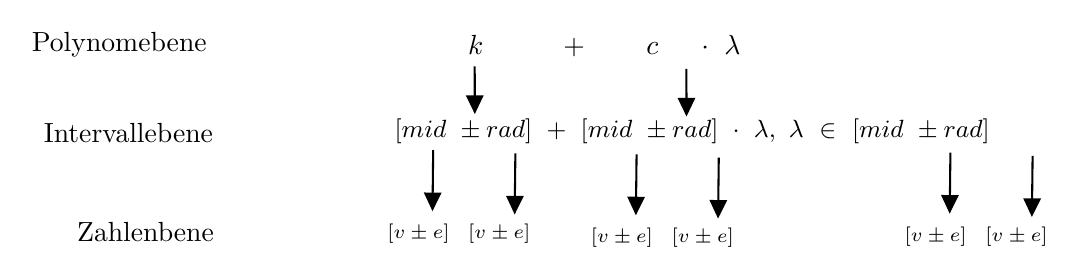
\begin{tikzpicture}[x=0.75pt,y=0.75pt,yscale=-1,xscale=1]
%uncomment if require: \path (0,300); %set diagram left start at 0, and has height of 300

%Straight Lines [id:da29898159624783616] 
\draw    (281.07,90.5) -- (280.77,116.88) ;
\draw [shift={(280.73,119.88)}, rotate = 270.65] [fill={rgb, 255:red, 0; green, 0; blue, 0 }  ][line width=0.08]  [draw opacity=0] (8.93,-4.29) -- (0,0) -- (8.93,4.29) -- cycle    ;
%Straight Lines [id:da1335093356184387] 
\draw    (320.67,92.1) -- (320.37,118.48) ;
\draw [shift={(320.33,121.48)}, rotate = 270.65] [fill={rgb, 255:red, 0; green, 0; blue, 0 }  ][line width=0.08]  [draw opacity=0] (8.93,-4.29) -- (0,0) -- (8.93,4.29) -- cycle    ;
%Straight Lines [id:da1340726243132735] 
\draw    (379.07,92.5) -- (378.77,118.88) ;
\draw [shift={(378.73,121.88)}, rotate = 270.65] [fill={rgb, 255:red, 0; green, 0; blue, 0 }  ][line width=0.08]  [draw opacity=0] (8.93,-4.29) -- (0,0) -- (8.93,4.29) -- cycle    ;
%Straight Lines [id:da9182990047680641] 
\draw    (418.67,94.1) -- (418.37,120.48) ;
\draw [shift={(418.33,123.48)}, rotate = 270.65] [fill={rgb, 255:red, 0; green, 0; blue, 0 }  ][line width=0.08]  [draw opacity=0] (8.93,-4.29) -- (0,0) -- (8.93,4.29) -- cycle    ;
%Straight Lines [id:da04610901450657834] 
\draw    (530.27,91.7) -- (529.97,118.08) ;
\draw [shift={(529.93,121.08)}, rotate = 270.65] [fill={rgb, 255:red, 0; green, 0; blue, 0 }  ][line width=0.08]  [draw opacity=0] (8.93,-4.29) -- (0,0) -- (8.93,4.29) -- cycle    ;
%Straight Lines [id:da7044032296577734] 
\draw    (569.87,93.3) -- (569.57,119.68) ;
\draw [shift={(569.53,122.68)}, rotate = 270.65] [fill={rgb, 255:red, 0; green, 0; blue, 0 }  ][line width=0.08]  [draw opacity=0] (8.93,-4.29) -- (0,0) -- (8.93,4.29) -- cycle    ;
%Straight Lines [id:da7628093943540135] 
\draw    (301.07,50.1) -- (301.12,70.08) ;
\draw [shift={(301.13,73.08)}, rotate = 269.84000000000003] [fill={rgb, 255:red, 0; green, 0; blue, 0 }  ][line width=0.08]  [draw opacity=0] (8.93,-4.29) -- (0,0) -- (8.93,4.29) -- cycle    ;
%Straight Lines [id:da9018979196177348] 
\draw    (403.07,51.3) -- (403.12,71.28) ;
\draw [shift={(403.13,74.28)}, rotate = 269.84000000000003] [fill={rgb, 255:red, 0; green, 0; blue, 0 }  ][line width=0.08]  [draw opacity=0] (8.93,-4.29) -- (0,0) -- (8.93,4.29) -- cycle    ;

% Text Node
\draw (86.2,32) node [anchor=north west][inner sep=0.75pt]   [align=left] {Polynomebene};
% Text Node
\draw (92,76) node [anchor=north west][inner sep=0.75pt]   [align=left] {Intervallebene};
% Text Node
\draw (108,124) node [anchor=north west][inner sep=0.75pt]   [align=left] {Zahlenbene};
% Text Node
\draw (296.4,33.8) node [anchor=north west][inner sep=0.75pt]    {$k\ \ \ \ \ \ \ \ +\ \ \ \ \ \  c\ \ \ \ \cdot \ \lambda $};
% Text Node
\draw (261,74) node [anchor=north west][inner sep=0.75pt]  [font=\small]  {$\left[\text{mid} \ \pm \text{rad}\right] \ +\ \left[\text{mid} \ \pm \text{rad}\right] \ \cdot \ \lambda ,\ \lambda \ \in \ \left[\text{mid} \ \pm \text{rad}\right]$};
% Text Node
\draw (257.5,124.6) node [anchor=north west][inner sep=0.75pt]  [font=\scriptsize]  {$\left[\text{v} \pm \text{e}\right] \ \ \left[\text{v} \pm \text{e}\right]$};
% Text Node
\draw (355.5,126.6) node [anchor=north west][inner sep=0.75pt]  [font=\scriptsize]  {$\left[\text{v} \pm \text{e}\right] \ \ \left[\text{v} \pm \text{e}\right]$};
% Text Node
\draw (506.7,125.8) node [anchor=north west][inner sep=0.75pt]  [font=\scriptsize]  {$\left[\text{v} \pm \text{e}\right] \ \ \left[\text{v} \pm \text{e}\right]$};


\end{tikzpicture}
